%!TEX root = paper.tex

To analyze the 1-dimensional problem, we will derive a group of sequences from the original collision sequence, which we will call the $\beta$ group. This group will allow us to validate any collision sequence. The first sequence in this group is defined below.

\begin{definition}
	Given a collision sequence $\alpha$, define a sequence $\beta^{(0)}$ where each element $\beta^{(0)}_i$ is the number of h's between the $i^{th}$ and $(i+1)^{th}$ v in $\alpha$. From Lemma \ref{lem:interval-ticks}, each element in $\beta^{(0)}$ can be one of two different values, which we will refer to as $\beta^{(0)}_{min}, \beta^{(0)}_{max}$.
\end{definition}

Graphically, $\beta^{(0)}_i$ represents the number of tick marks in each interval. An example sequence is shown in Figure \ref{fig:beta-sequence}.

\begin{figure}[H]
  \begin{center}
    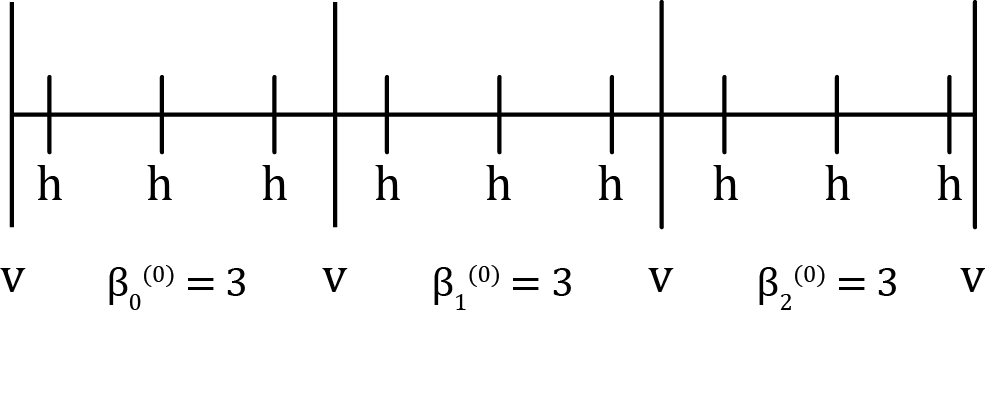
\includegraphics[keepaspectratio]{1d_mapping_3}
  \end{center}
  \vspace{-.2in} % corrects bad spacing
  \caption{\label{fig:beta-sequence} An example $\beta^{(0)}$ sequence.}
\end{figure}

 We will also need a new sequence $\delta^{(0)}$ where each element is spaced $-1 \, \cbracket{\frac{m}{1}}$ apart. $\delta^{(0)}$ will also include an offset of $(1-y_0)$ for reasons that will become clear shortly. In terms of our $\beta$ group, $\cbracket{\frac{m}{1}}$ can be written as 

\begin{equation}
  \cbracket{\frac{m}{1}} = \frac{m}{1} - \beta^{(0)}_{min}
\end{equation}

So, we can write $\delta^{(0)}$ in terms of $\beta$

\begin{definition}
  $\delta^{(0)}$ is defined more precisely as

  \begin{align}\label{delta_beta}
    \delta^{(0)}_i \coloneqq \begin{cases}
      1-y_0 \qquad &\text{for} \quad i = 0\\
      i (\beta^{(0)}_{min} - m) + (1-y_0) \qquad &\text{for} \quad i \ge 1
    \end{cases}
  \end{align}
\end{definition}

Visually, each element $\delta^{(0)}_i$ is the signed distance between the beginning of the $i^{th}$ interval and the $(i \, \beta^{(0)}_{min})^{th}$ tick mark. Figure \ref{fig:delta-sequence} shows the $\delta^{(0)}_i$ sequence on top of the original parametric representation (top) as well as by itself (bottom).

\begin{figure}[H]
  \begin{center}
    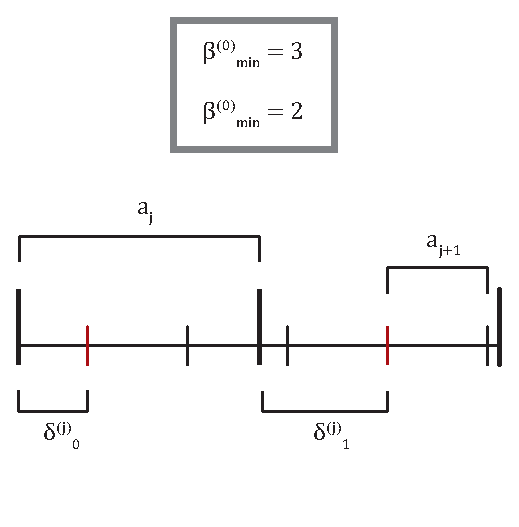
\includegraphics[keepaspectratio]{1d_mapping_4}
  \end{center}
  \vspace{-.2in} % corrects bad spacing
  \caption{\label{fig:delta-sequence} Generating the $\delta^{(0)}$ sequence.}
\end{figure}

Our next step is to define $\beta^{(j)}, \delta^{(j)}$ for $j \ge 1$, which will be done in a inductive manner. Before continuing, lets create a third sequence, that we will call $a$.

\begin{definition}
  \begin{equation}
    a_j \coloneqq \begin{cases}
      m \qquad &\text{for} \quad i = -2\\
      1 \qquad &\text{for} \quad i = -1\\
      a_{j-2} - \beta^{(j)} a_{j-1} &\qquad \text{for} \quad i \ge 0
    \end{cases}
  \end{equation}
\end{definition}

$a_{-2}, a_{-1}$ are the interval size and tick spacing in our original problem. $a_0$ is the spacing of elements of $\delta^{(0)}$. $a_j$ for $j \ge 1$ will represent the spacing of elements of $\delta^{(j)}$ sequences which will be defined shortly. For the moment, the reader should assume that, given some $j$, $\delta^{(j-1)}$ exists, and l

\begin{figure}[H]
  \begin{center}
    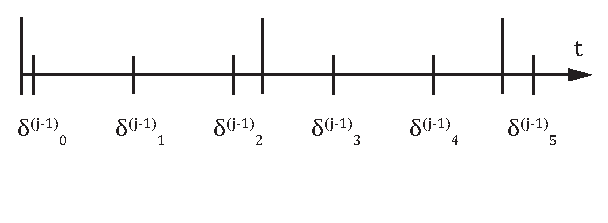
\includegraphics[keepaspectratio]{1d_mapping_6}
  \end{center}
  \vspace{-.2in} % corrects bad spacing
  \caption{\label{fig:delta-sequence-2} An example $\delta^{(0)}$ sequence.}
\end{figure}

We will now build off of the $\beta^{(0)}$ sequence, and extend the $\beta$ group inductively.

\begin{definition}
  \label{def:beta-definition}
  Given a $j > 0$ and a collision sequence $\alpha$, assume that $\beta^{(j-1)}$ is defined and each element in the sequence is either $\beta^{(j-1)}_{min}$ or $\beta^{(j-1)}_{max}$. The sequence $\beta^{(j)}$ is defined such that each element $\beta^{(j)}_i$ is 1 more than the number of occurrences of $\beta^{(j-1)}_{max}$ between the $i^{th}$ and $(i+1)^{th}$ occurrence of $\beta^{(j-1)}_{min}$ in the $\beta^{(j-1)}$ sequence. From Lemma \ref{lem:interval-ticks}, each element in $\beta^{(j)}$ can be one of two different values, which we will refer to as $\beta^{(j)}_{min}, \beta^{(j)}_{max}$.

  If, for some $j_f$, the length of $\beta^{(j_f-1)}$ is 1, then $\beta^{(j_f-1)}$ is called the terminating $\beta$ sequence, and all subsequent $\beta^{(j)}$ for $j \ge j_f$ are undefined.
\end{definition}

$\beta^{(j)}$ is much simpler to understand visually. A visualization representation is formed using the following rules:

\begin{enumerate}
  \item Divide the number line into regular intervals of length $a_{j}$.
  \item $\beta^{(j-1)}_{min}$ are represented as tick marks on the number line with a regular spacing $a_{j+1}$.
  \item There is exactly one $\beta^{(j-1)}_{min}$ tick mark in each interval.
  \item In each interval, all the $\beta^{(j-1)}_{max}$ terms come before the $\beta^{(j-1)}_{min}$ term.
\end{enumerate}

Then $\beta^{(j)}_i$ is the number of tick marks in each interval. An example $\beta^{(j-1)}$ visual representation is shown in Figure \ref{fig:beta-sequence-j}.

\begin{figure}[H]
  \begin{center}
    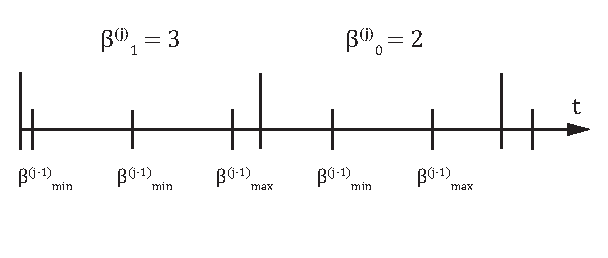
\includegraphics[keepaspectratio]{1d_mapping_7}
  \end{center}
  \vspace{-.2in} % corrects bad spacing
  \caption{\label{fig:beta-sequence-j} A general $\beta^{(j)}$ sequence.}
\end{figure}


Lastly, we need to extend our $\delta$ group, such that each $\delta^{(j)}_i$ is the distance between the $(i \, \beta^{(j)}_{max})^{th}$ tick mark and the beginning of the $i^{th}$ interval in the $\beta^{(j)}$ visual representation.

\begin{definition}
  $\delta^{(j)}$ is defined more precisely as

  \begin{align}\label{delta_beta}
    \delta^{(j)}_i \coloneqq \begin{cases}
      1-y_0 \qquad &\text{for} \quad i = 0\\
      i (\beta^{(j)}_{min} * a_{j-1} - a_{j-2}) + (1-y_0) \qquad &\text{for} \quad i \ge 1
    \end{cases}
  \end{align}
\end{definition}

The number of tick marks in the $i^{th}$ interval is thus equal to $\beta^{(j)}_{max}$ plus the number of tick marks included in the $\delta^{(j)}_i$ interval minus the number of tick marks included in the $\delta^{(j)}_{i+1}$ interval. More precisely

\begin{align}\label{eq:beta_i}
  \beta^{(j)}_i = \floor{\delta^{(j)}_i} + \beta^{(j)}_{max} - \floor{\delta^{(j)}_{i+1}}
\end{align}
